\begin{table}[!t]
\centering
\caption{Held-out quality and re-retrieval (\%, $n=1{,}000$). The three calibrated gates share a 20\% dev target.}
\label{tab:quality}
\footnotesize
\setlength{\tabcolsep}{3.5pt}
\begin{tabular}{lrrrr}
\hline
Policy & Answer F1 & EM & Supp-F1 & Retrieval \\
\hline
Never & 50.85 & 40.10 & 47.51 & 0.0 \\
Always & 57.66 & 46.20 & 52.38 & 100.0 \\
NLI threshold & 53.89 & 42.70 & 50.15 & 21.9 \\
Crisp & 54.36 & 43.00 & 50.22 & 20.9 \\
Fuzzy & 54.42 & 43.20 & 50.24 & 23.0 \\
Full-context & 64.27 & 50.20 & 54.90 & 0.0 \\
A/B Oracle & 60.61 & 49.20 & 51.35 & 12.3 \\
\hline
\end{tabular}
\end{table}

\begin{table}[!t]
\centering
\caption{Real-path cost on 32 shared questions per policy. Token counts include the answer and selector calls.}
\label{tab:cost}
\footnotesize
\setlength{\tabcolsep}{3.5pt}
\begin{tabular}{lrrrr}
\hline
Policy & Mean (s) & P90 (s) & Input & Output \\
\hline
Never & 19.26 & 23.76 & 697.8 & 27.3 \\
Always & 19.13 & 22.56 & 814.7 & 26.4 \\
NLI threshold & 23.32 & 28.87 & 810.2 & 30.8 \\
Crisp & 22.83 & 28.61 & 800.9 & 30.3 \\
Fuzzy & 23.36 & 28.65 & 810.2 & 30.8 \\
Full-context & 24.91 & 29.67 & 1916.8 & 27.8 \\
\hline
\end{tabular}
\end{table}

\begin{table}[!t]
\centering
\caption{Question-level paired answer-F1 contrasts in percentage points. Intervals are individual 95\% percentile bootstrap intervals.}
\label{tab:paired}
\footnotesize
\setlength{\tabcolsep}{3.5pt}
\begin{tabular}{lrr}
\hline
Contrast & Difference & 95\% interval \\
\hline
Fuzzy $-$ Crisp & +0.064 & [-0.365, +0.517] \\
Fuzzy $-$ NLI threshold & +0.531 & [+0.155, +0.994] \\
Fuzzy $-$ Never & +3.576 & [+2.265, +4.914] \\
A/B Oracle $-$ Never & +9.758 & [+8.059, +11.471] \\
Full-context $-$ Fuzzy & +9.841 & [+7.098, +12.614] \\
\hline
\end{tabular}
\end{table}

\begin{table}[!t]
\centering
\caption{Gate selection and ablations. A positive case has strictly higher branch B answer F1. Rate and answer F1 are percentages.}
\label{tab:gate}
\footnotesize
\setlength{\tabcolsep}{3.5pt}
\begin{tabular}{lrrrrr}
\hline
Policy & F1 & Rate & P & R & Gate F1 \\
\hline
NLI threshold & 53.89 & 21.9 & 0.224 & 0.398 & 0.287 \\
Crisp & 54.36 & 20.9 & 0.258 & 0.439 & 0.325 \\
Fuzzy & 54.42 & 23.0 & 0.243 & 0.455 & 0.317 \\
Fuzzy w/o NLI & 56.82 & 66.0 & 0.152 & 0.813 & 0.255 \\
Fuzzy w/o bridge & 53.79 & 20.7 & 0.227 & 0.382 & 0.285 \\
\hline
\end{tabular}
\end{table}

\begin{table}[!t]
\centering
\caption{Answer-F1 changes versus Never across all 1,000 test questions. An untriggered gate preserves A and counts as a tie.}
\label{tab:changes}
\footnotesize
\setlength{\tabcolsep}{3.5pt}
\begin{tabular}{lrrr}
\hline
Policy & Improved & Tie & Degraded \\
\hline
Always & 123 & 827 & 50 \\
NLI threshold & 49 & 934 & 17 \\
Crisp & 54 & 932 & 14 \\
Fuzzy & 56 & 927 & 17 \\
A/B Oracle & 123 & 877 & 0 \\
\hline
\end{tabular}
\end{table}

\begin{figure*}[!t]
\centering
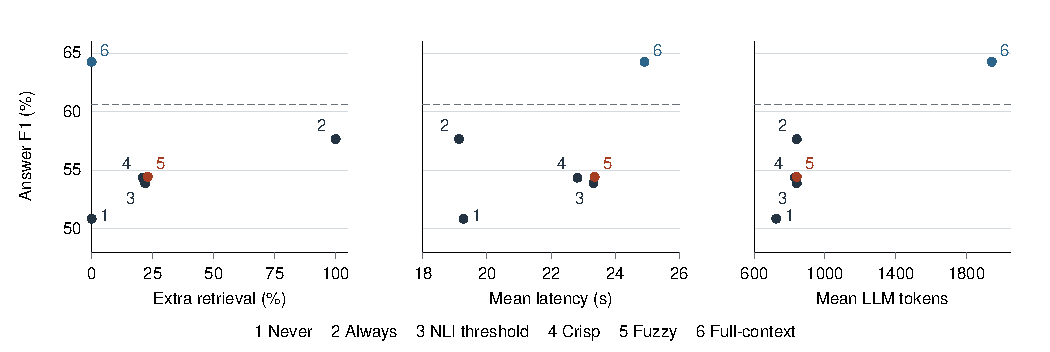
\includegraphics[width=.98\textwidth]{quality_cost.pdf}
\caption{Held-out answer F1 against test re-retrieval rate and live mean costs. The dashed line marks the A/B Oracle F1. Re-retrieval rate uses the full test set. The latency and token axes use 32 shared questions per policy.}
\label{fig:quality-cost}
\end{figure*}
